\documentclass{article}

\usepackage{graphicx}
\usepackage{fancyhdr}
\usepackage[margin=1in]{geometry}
\usepackage{listings}
\usepackage[hidelinks]{hyperref}
%\usepackage{subfigure}
\usepackage{subcaption}

\usepackage{amsmath}
\usepackage{subcaption}
\usepackage{float}
\usepackage{booktabs}

\hypersetup{
	colorlinks=true,
	linkcolor=teal,
	filecolor=magenta,      
	urlcolor=teal,
	citecolor = teal
}
\usepackage{xcolor}
\usepackage{xepersian}
\setlength\headheight{28pt} 
\settextfont[
    Path = ./font/, % specify the path to the font files
    Scale = 1.3,
    UprightFont = XB Niloofar, % Regular font
    BoldFont = XB NiloofarBd,       % Bold font
    ItalicFont = XB NiloofarIt,   % Italic font
    BoldItalicFont = XB NiloofarBdIt % Bold Italic font if available
]{XB Niloofar}
\setlatintextfont[Scale=1.3]{Times New Roman}
\renewcommand{\baselinestretch}{1.5}
\pagestyle{fancy}
\fancyhf{}
\rhead{
\includegraphics[width=1cm]{img/Logo.png} 
	یادگیری ماشین
	-
	مینی پروژه شماره 2}
\lhead{\thepage}
\rfoot{سیدمحمد حسینی}
\lfoot{9821253}
\renewcommand{\headrulewidth}{1pt}
\renewcommand{\footrulewidth}{1pt}
\renewcommand{\lstlistingname}{Code}

\definecolor{codegreen}{rgb}{0,0.6,0}
\definecolor{codegray}{rgb}{0.5,0.5,0.5}
\definecolor{codepurple}{rgb}{0.58,0,0.82}
\definecolor{backcolour}{rgb}{0.95,0.95,0.92}

\lstdefinestyle{mystyle}{
	backgroundcolor=\color{backcolour},   
	commentstyle=\color{codegreen},
	keywordstyle=\color{magenta},
	numberstyle=\tiny\color{codegray},
	stringstyle=\color{codepurple},
	basicstyle=\ttfamily\footnotesize,
	breakatwhitespace=false,         
	breaklines=true,                 
	captionpos=b,                    
	keepspaces=true,                 
	numbers=left,                    
	numbersep=5pt,                  
	showspaces=false,                
	showstringspaces=false,
	showtabs=false,                  
	tabsize=2
}

\lstset{style=mystyle}

\begin{document}
	
	\begin{titlepage}
\begin{center}
\defpersianfont\nast[Path={./font/}, Scale=2]{IranNastaliq}
\centerline{{
\includegraphics[width=5cm]{img/Logo.png}}}
\centerline{\textcolor[rgb]{0,0,0.5}{\nast \large  دانشگاه صنعتی خواجه نصیرالدین طوسی}}
\centerline{\textcolor[rgb]{0,0,0.5}{\nast \bfseries دانشکدۀ مهندسی برق - گروه مهندسی کنترل}}

\vfill
        
\Huge
\textbf{یادگیری ماشین}\\
\textbf{پاسخ مینی پروژه دوم}\\
        
\vfill
\large
    نام و نام خانوادگی:  سیدمحمد حسینی\\
    شمارۀ دانشجویی: 9901399\\
    تاریخ: مهرماه 1402\\

\href{https://github.com/mamdaliof/MachineLearning2024W}{GitHub}

\href{https://drive.google.com/drive/folders/10-8uiqpIUbC2HcEtwjqP1IAix46nCrbL?usp=sharing}{Google Drive}


\end{center}
\end{titlepage}

	
	\tableofcontents \clearpage
	\listoffigures \clearpage
	\listoftables \clearpage
	\lstlistoflistings \clearpage
	\newpage

\section{پرسش2}

\subsection{قسمت اول}

\lr{lunar lander}
 فضاپیمایی است که برای فرود آمدن بر سطح ماه طراحی شده است و مأموریت آن فرود ایمن از مدار ماه به سطح ماه است. هدف اصلی این فضاپیما شامل طی کردن مسیر دقیق فرود و فرود ایمن و نرم است که نیازمند سیستم‌های راهنمایی پیشرفته، ناوبری دقیق و طراحی ساختاری قوی است. سیستم پیشرانه که شامل موتورهای اصلی فرود و موتورهای کنترل وضعیت جانبی و کوچکتر است که نقش مهمی در کنترل سرعت فرود و جهت‌گیری ایفا می‌کند. \lr{lunar lander} همچنین دارای پایه‌های فرود برای کاهش اثر ضربه و تضمین پایداری هستند. 
 
 یادگیری تقویتی (RL) می‌تواند برای مسئله کنترل یک
 \lr{lunar lander}
استفاده شود. در این زمینه، RL شامل آموزش یک Agent برای یادگیری یک Policy بهینه برای فرود ایمن و کارآمد م
\lr{lunar lander}
 است. اجزای اصلی یک مسئله RL شامل فضای حالت، فضای عمل و سیستم پاداش است که این موارد به شرح زیر می‌باشند.
 
 \textbf{فضای حالت}
 
 فضای حالت تمام حالات ممکن را که فرودگر قمری می‌تواند در آن‌ها باشد، نشان می‌دهد. برای یک \lr{lunar lander} فضای حالت می‌تواند شامل موارد زیر باشد:
  \begin{itemize}
 \item مختصات عمودی و افقی فرودگر.
 \item مولفه‌های سرعت در جهت‌های افقی و عمودی.
 \item زاویه فرودگر نسبت به عمود.
 \item سرعت زاویه‌ای فرودگر.
 \item وضعیت پایه‌های فرودگر
  \end{itemize}
 هر حالت نمایانگر شرایط فرودگر در یک گام زمانی معین است.
 
 \textbf{فضای عمل}
 
 فضای عمل تمام Actions ممکن را که Agent می‌تواند انجام دهد، نشان می‌دهد. برای یک \lr{lunar lander} فضای عمل می‌تواند شامل موارد زیر باشد:
\begin{itemize}
 \item توان موتور اصلی.
 \item توان موتور چپ.
 \item توان موتور راست.
 \item انجام ندادن هیچ کاری.
\end{itemize}

 این Actions نیروی پیشرانه و جهت‌گیری فرودگر را کنترل می‌کنند.
 
 \textbf{سیستم پاداش}
 
 سیستم پاداش بازخوردی به Agent بر اساس Actions آن و تغییرات حالت ناشی از آن‌ها ارائه می‌دهد. برای یک \lr{lunar lander} سیستم پاداش ممکن است به این صورت طراحی شود:
 \begin{itemize}

 \item پاداش مثبت برای دستیابی به فرود ایمن با سرعت کم.
 \item پاداش منفی برای فرودهای سخت یا سقوط‌ها.
 \item پاداش منفی برای مصرف سوخت زیاد.
 \item پاداش مثبت برای حفظ جهت‌گیری پایدار.
 \item پاداش منفی کوچک برای هر گام زمانی برای تشویق فرود سریع‌تر.
   \end{itemize}
 سیستم پاداش Agent را تشویق می‌کند تا Policy‌هایی را بیاموزد که منجر به فرودهای ایمن، کارآمد و پایدار شود.
 \cite{xu_2024}

\subsection{قسمت دوم}

ابتدا به بررسی بلاک‌های کد می‌پردازیم.
\begin{LTR}
	\begin{lstlisting}[language=Python, caption=Deep Neural Network]
# DQN
import torch.nn as nn
import torch.nn.functional as F

class DeepQNetwork(nn.Module):
    def __init__(self, state_size, action_size) -> None:
        super(DeepQNetwork, self).__init__()
        # TODO: define the architecture
        # NOTE: input=observation/state, output=action
        net_list = nn.ModuleList([
            torch.nn.Linear(state_size, 512),
            torch.nn.ReLU(),
            torch.nn.LayerNorm(512),
            torch.nn.Dropout(0.1),
            torch.nn.Linear(512, 512),
            torch.nn.ReLU(),
            torch.nn.LayerNorm(512),
            torch.nn.Dropout(0.1),
            torch.nn.Linear(512, 512),
            torch.nn.ReLU(),
            torch.nn.Linear(512, action_size)
        ])
        self.net = torch.nn.Sequential(*net_list).to(device)

    def forward(self, x):
        # TODO: forward propagation
        # NOTE: use ReLu for activation function in all layers
        # NOTE: last layer has no activation function (predict action)
        # ReLU is created in init, no need here
        x.to(device)
        x = self.net(x)
        return x
	\end{lstlisting}
\end{LTR}
کد فوق یک شبکه عصبی عمیق را ایجاد می‌کند که به موجب آن 4 لایه خطی به همراه 3 لایه غیر خطی ایجاد شده است تا ماتریس پاداش را پیشبینی کند.


\begin{LTR}
	\begin{lstlisting}[language=Python, caption=Agent Class]
# DQN agent
import numpy as np
import torch
import torch.nn as nn
import torch.nn.functional as F
import torch.optim as optim

class DQNAgent():
    # NOTE: DON'T change initial values
    def __init__(self, state_size, action_size, batch_size,
                 gamma=0.99, buffer_size=25000, alpha=1e-4):
        # network parameter
        self.state_size = state_size
        self.action_size = action_size

        # hyperparameters
        self.batch_size = batch_size
        self.gamma = gamma

        # experience replay
        self.experience_replay = ExperienceReplay(buffer_size)

        # network
        self.value_net = DeepQNetwork(state_size, action_size).to(device)

        # optimizer
        # TODO: create adam for optimizing network's parameter (learning rate=alpha)
        self.optimizer = optim.Adam(self.value_net.parameters(), lr=alpha)

    def take_action(self, state, eps=0.0):
        # TODO: take action using e-greedy policy
        # NOTE: takes action using the greedy policy with a probability of 1−𝜖 and a random action with a probability of 𝜖
        # NOTE:
        self.value_net.eval()
        if len(state) != 8 :
            state = state[0]
        rand_eps = random.random()
        if rand_eps > eps:
            with torch.no_grad():
                # print(state)
                return torch.argmax(self.value_net(torch.tensor(state).to(device))).detach().cpu().numpy()
        else:
            return np.random.randint(0, self.action_size)

    def update_params(self):
        if len(self.experience_replay) < self.batch_size:
            return
        # transition batch
        batch = Transition(*zip(*self.experience_replay.sample(self.batch_size)))

        temp = []
        for indx in range(len(batch.state)):
            if len(batch.state[indx]) != 8:
                temp.append(batch.state[indx][0])
            else:
                temp.append(batch.state[indx])
        state_batch = torch.from_numpy(np.vstack(temp)).float().to(device)  # [8, 8]
        action_batch = torch.tensor(np.vstack(batch.action)).long().to(device) # [8, 1]
        next_state_batch = torch.from_numpy(np.vstack(batch.next_state)).float().to(device) # [8, 8]
        reward_batch = torch.tensor(np.vstack(batch.reward)).float().to(device) # [8, 1]
        done_batch = torch.tensor(np.vstack(batch.done)).to(device)

        # calculate loss w.r.t DQN algorithm
        self.value_net.train()
        # STEP1
        q_expected = self.value_net(state_batch).gather(1, action_batch)
        # TODO: compute the expected Q values [y]
        # STEP2
        # TODO: compute Q values [Q(s_t, a)]
        q_targets_next = self.value_net(next_state_batch).detach().max(1)[0].unsqueeze(1)
        q_targets = reward_batch + (self.gamma * q_targets_next * (1 - done_batch*1))
        # STEP3
        # TODO: compute mse loss
        loss = nn.functional.mse_loss(q_expected, q_targets)
        # TODO: optimize the model
        # NOTE: DON'T forget to set the gradients to zeros
        self.optimizer.zero_grad()
        loss.backward()
        self.optimizer.step()

    def save(self, fname):
        # TODO: save checkpoint
        torch.save(self.value_net, fname)

    def load(self, fname, device):
        # TODO: load checkpoint
        self.value_net = torch.load(fname, device)
	\end{lstlisting}
\end{LTR}

در این بخش، کلاس \texttt{DQNAgent} تعریف می‌شود که Agent مربوط به DQN را پیاده‌سازی می‌کند. این کلاس مسئول مدیریت شبکه عصبی، اجرای  
\lr{Policy $\epsilon$-Greedy}
، به‌روزرسانی پارامترهای شبکه و ذخیره و بارگذاری مدل است.

\subsubsection{تعریف متغیرها و مقادیر اولیه}

در ابتدای کلاس، مقادیر اولیه و پارامترهای شبکه تعریف می‌شوند. این شامل اندازه State
 (\texttt{state\_size})، اندازه Action
 (\texttt{action\_size})، اندازه 
 Batch
  (\texttt{batch\_size})، (\texttt{gamma})، اندازه Buffer  (\texttt{buffer\_size}) و نرخ یادگیری (\texttt{alpha}) است.



در ادامه
شبکه عصبی (\texttt{DeepQNetwork}) برای پیش‌بینی مقادیر Q و بهینه‌ساز \texttt{Adam} با نرخ یادگیری $\alpha$ تعریف می‌شوند.



\subsubsection{متد \texttt{take\_action}}

این تابع برای انتخاب اقدام با استفاده از
 \lr{Policy $\epsilon$-Greedy} 
 استفاده می‌شود. با احتمال $1 - \epsilon$، اقدام بهینه انتخاب می‌شود و با احتمال $\epsilon$، یک اقدام تصادفی انتخاب می‌شود.


\subsubsection{متد \texttt{update\_params}}

این تابع پارامترهای شبکه عصبی را به‌روزرسانی می‌کند. اگر تعداد تجربیات کمتر از \texttt{batch\_size} باشد، تابع متوقف می‌شود. در ادامه تجربیات نمونه‌گیری شده و به فرمت مناسب برای استفاده در شبکه عصبی تبدیل می‌شوند.\\
حال مقادیر Q مورد انتظار (\texttt{q\_expected}) و سپس مقادیر هدف Q (\texttt{q\_targets}) محاسبه می‌شوند. سپس با استفاده از (MSE) تابع هزینه محاسبه شده و مدل بهینه‌سازی می‌شود.




\begin{LTR}
	\begin{lstlisting}[language=Python, caption=Train]
# training phase

# TODO: create agent
agent = DQNAgent(state_size, action_size, batch_size=BATCH_SIZE)

crs = np.zeros(n_episodes) # cummulative rewards
crs_recent = deque(maxlen=25) # recent cummulative rewards

# training loop
for i_episode in range(1, n_episodes+1):
    # TODO: initialize the environment and state
    if i_episode % 50 == 0:
        env = RecordVideo(gym.make("LunarLander-v2"), f"./DQN/batch{BATCH_SIZE}/eps{i_episode}")
    else:
        env = gym.make("LunarLander-v2")
    state = env.reset()
    done = False
    cr = 0 # episode cummulative rewards
    while not done:
        env.render()
        # TODO: select and perform an action
        action = agent.take_action(state, eps)
#         print(action)
        # Modify the unpacking to handle the extra value if present
        result = env.step(action)
        if len(result) == 5:
            next_state, reward, done, truncated, info = result
        else:
            next_state, reward, done, info = result
        # TODO: store transition in experience replay
        agent.experience_replay.store_trans(state, action, next_state, reward, done)
        # TODO: update agent
        agent.update_params()
        # TODO: update current state and episode cummulative rewards
        # print("next" ,next_state)
        state = next_state
        cr += reward

    # TODO: decay epsilon
    eps = eps * eps_decay_rate
    eps = max(eps, eps_end)
    # TODO: update current cummulative rewards and recent cummulative rewards
    crs[i_episode - 1] = cr
    crs_recent.append(cr)
    # TODO: save agent every 50 episodes
    if i_episode % 50 == 0:
        agent.save(f"q_net_batch{BATCH_SIZE}_eps{i_episode}.pt")

    # print logs
    print('\rEpisode {}\tAverage Reward: {:.2f}\tEpsilon: {:.2f}'.format(i_episode, np.mean(crs_recent), eps), end="")
    if i_episode % 25 == 0:
        print('\rEpisode {}\tAverage Reward: {:.2f}\tEpsilon: {:.2f}'.format(i_episode, np.mean(crs_recent), eps))
	\end{lstlisting}
\end{LTR}



\subsubsection{Training}

در این بخش، کدهای مربوط به بخش Training توضیح داده می‌شود. این فاز شامل ایجاد Agent، اجرای حلقه آموزش، انتخاب Actions، به‌روزرسانی پارامترها، و ذخیره مدل است.


در گام نخست Agent مد نظر ما با مقادیر اولیه متناسب با مسئله ایجاد می‌شود. در ادامه 
متغیر \texttt{crs} برای ذخیره پاداش‌های تجمعی هر اپیزود و \texttt{crs\_recent} برای ذخیره پاداش‌های تجمعی اخیر تعریف می‌شود.\\
حلقه آموزش برای تعداد اپیزودهای مشخص شده (\texttt{n\_episodes}) اجرا می‌شود تا Agent پاسخ بهینه به سمئله را پیدا کند.
در این حلقه آموزش به ازای هر اپیزود، محیط و حالت اولیه مقداردهی می‌شوند. هر 50 اپیزود، محیط برای  RecordVideo تنظیم می‌شود.

تا زمانی که اپیزود به پایان نرسیده است، حلقه steps اجرا می‌شود. در هر گام، محیط رندر می‌شود و Agent یک اقدام انتخاب می‌کند.
نتیجه اقدام انجام شده دریافت می‌شود و انتقال در تجربه‌های Agent ذخیره می‌شود.
پارامترهای Agent به‌روزرسانی می‌شوند و حالت فعلی و پاداش‌های تجمعی اپیزود به‌روز می‌شوند.
پس از پایان اپیزود، مقدار \texttt{epsilon} کاهش می‌یابد تا به تدریج Agent کمتر به Actions تصادفی روی بیاورد.
پاداش‌های تجمعی اپیزود جاری و پاداش‌های تجمعی اخیر به‌روز می‌شوند.
هر 50 اپیزود، مدل Agent ذخیره می‌شود.


\subsubsection{نتایج}
نمودارهای زیر برای نمایش نتایج حاصله از آموزش مدل رسم شده‌اند.
\begin{figure}[H]
\centering
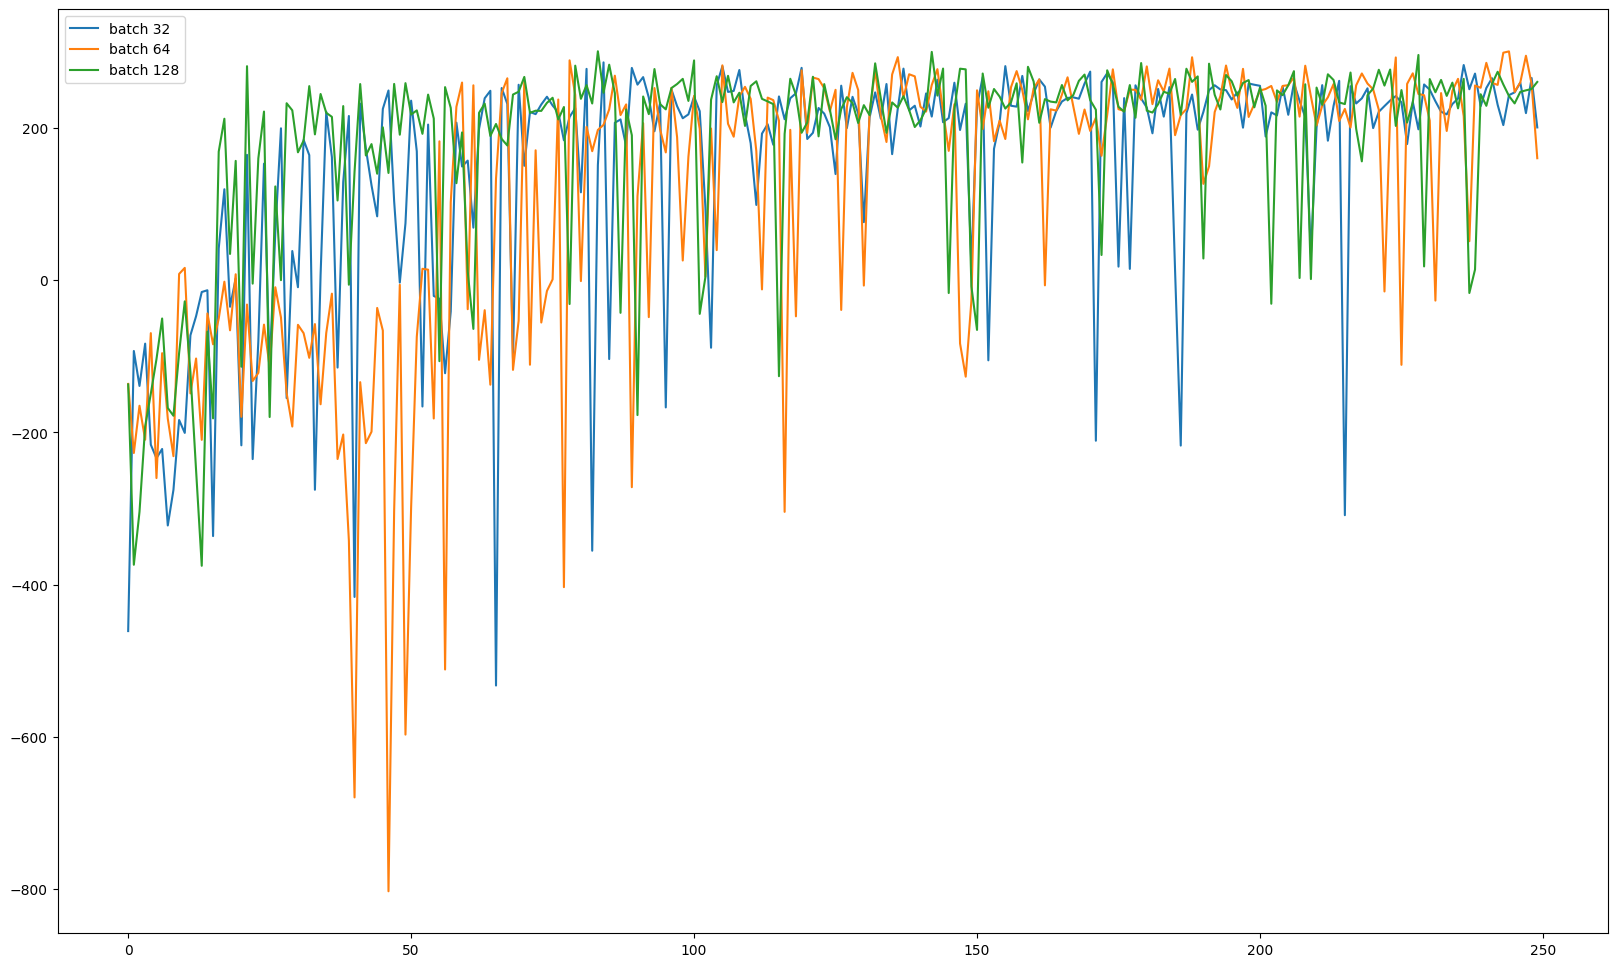
\includegraphics[width=1.0\linewidth]{img/result1}
\caption{نتایج به ازای تمام اپیزودها}
\label{fig:result1}
\end{figure}
\begin{figure}[H]
\centering
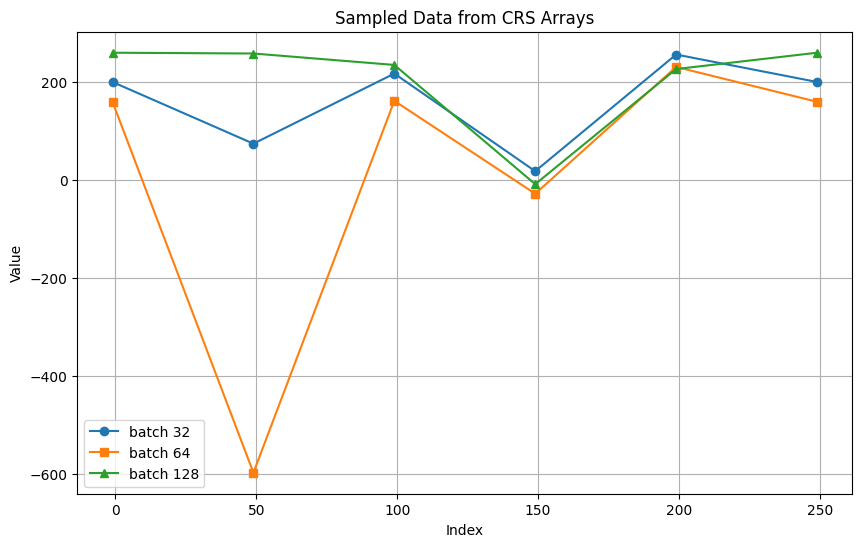
\includegraphics[width=1.0\linewidth]{img/result2}
\caption{نتایج به ازای هر 50 اپیزود}
\label{fig:result2}
\end{figure}
همانطور که انتظار می‌رفت نتاج به ازای بچ 128 زودتر همگرا شده است اما به ازای بچ 64 نتایج همگرایی ضعیفتری داشته است نسبت به حالتی که بچ 32 بوده است. بنابراین بهترین حالت مربوط به بچ128 بوده و به منظور توجه به سرعت همگرایی در اپیزود 50 بهترین مدل انتخاب می‌شود.

کد اجرایی به منظور ذخیره ویدیو از آموزش Agent همراه با یک ارور بوده که امکان حل آن وجود نداشت. ارور در فایل نوتبوک موجود می‌باشد.

\subsection{قسمت سوم}


در یادگیری تقویتی، DQN و DDQN دو روش محبوب برای یادگیری Q-مقادیر هستند. هر دو روش به منظور بهبود عملکرد Agent در انتخاب بهترین Actions در یک محیط مشخص توسعه داده شده‌اند. در اینجا تفاوت‌ها و شباهت‌های کلیدی بین DQN و DDQN را بررسی می‌کنیم.

\subsubsection{DQN}

\begin{itemize}
  \item \textbf{معماری:} DQN از یک شبکه عصبی عمیق برای تقریب Q-مقادیر استفاده می‌کند. این شبکه عصبی ورودی‌هایی شامل حالت‌های محیط را دریافت کرده و Q-مقادیر مربوط به هر اقدام ممکن را تولید می‌کند.
  \item \textbf{به‌روزرسانی Q-مقادیر:} در DQN، از یک شبکه هدف  استفاده می‌شود که کپی‌ای از شبکه اصلی (Q-Network) است و در فواصل زمانی منظم به‌روزرسانی می‌شود. این کار به پایداری یادگیری کمک می‌کند.
  \item \textbf{معادله به‌روزرسانی:} معادله به‌روزرسانی Q-مقادیر در DQN به صورت زیر است:
  \[
  Q(s, a) \leftarrow Q(s, a) + \alpha \left( r + \gamma \max_{a'} Q'(s', a') - Q(s, a) \right)
  \]
  که در آن \( Q'(s', a') \) مقدار Q پیش‌بینی شده توسط شبکه هدف است.
  \item \textbf{\lr{Over fitting}} در DQN، به دلیل استفاده از \(\max_{a'} Q(s', a')\) برای به‌روزرسانی Q-مقادیر، احتمال \lr{Over fitting}وجود دارد که می‌تواند منجر به پایداری کمتر در یادگیری شود.
\end{itemize}

\subsubsection{DDQN}

\begin{itemize}
  \item \textbf{معماری:} معماری شبکه عصبی در DDQN مشابه DQN است، با این تفاوت که در DDQN دو شبکه Q به‌صورت جداگانه به‌روزرسانی می‌شوند: یک شبکه Q اصلی و یک شبکه Q هدف.
  \item \textbf{به‌روزرسانی Q-مقادیر:} در DDQN، به‌روزرسانی Q-مقادیر به گونه‌ای اصلاح شده است که از \lr{Over fitting}جلوگیری شود. این کار با استفاده از شبکه Q اصلی برای انتخاب Actions و شبکه Q هدف برای محاسبه Q-مقادیر انجام می‌شود.
  \item \textbf{معادله به‌روزرسانی:} معادله به‌روزرسانی Q-مقادیر در DDQN به صورت زیر است:
  \[
  Q(s, a) \leftarrow Q(s, a) + \alpha \left( r + \gamma Q'(s', \arg\max_{a'} Q(s', a')) - Q(s, a) \right)
  \]
  که در آن \( Q(s', a') \) مقدار Q پیش‌بینی شده توسط شبکه Q اصلی است و \( Q'(s', \arg\max_{a'} Q(s', a')) \) مقدار Q پیش‌بینی شده توسط شبکه هدف با استفاده از اقدام انتخاب شده توسط شبکه Q اصلی است.

\end{itemize}

\begin{figure}[H]
\centering
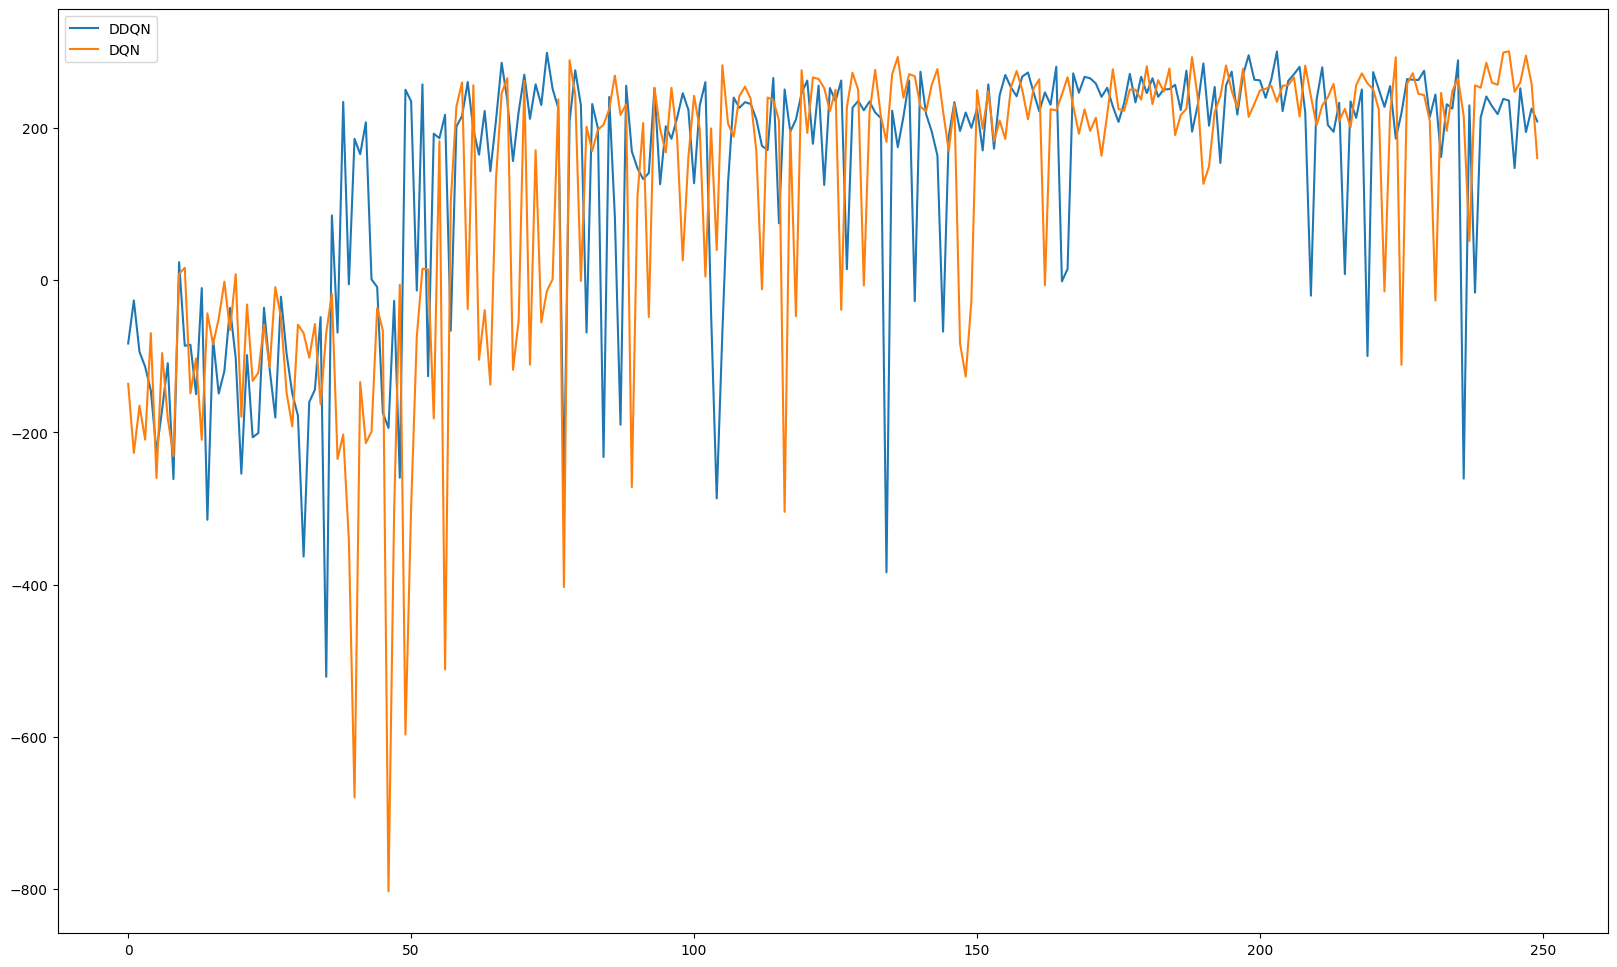
\includegraphics[width=1.0\linewidth]{img/result3}
\caption{مقایسه DQN و DDQN}
\label{fig:result3}
\end{figure}

\begin{figure}[H]
\centering
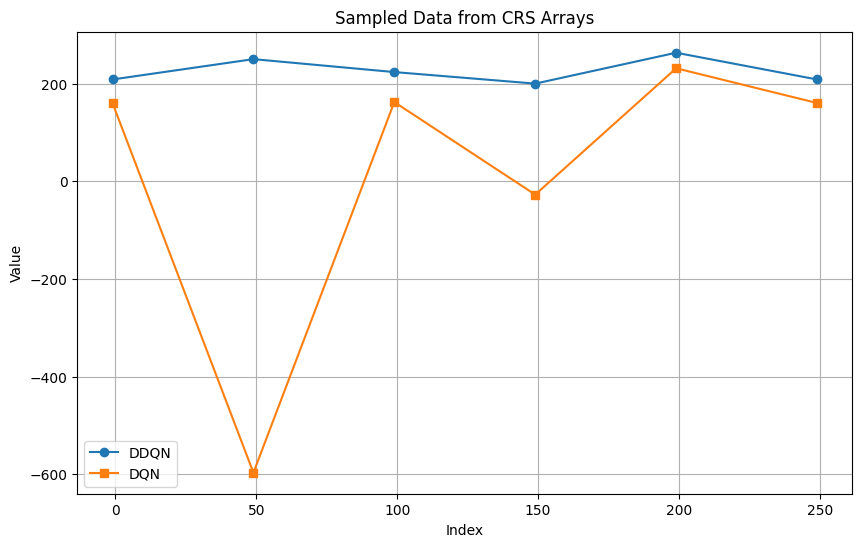
\includegraphics[width=1.0\linewidth]{img/result4}
\caption{مقایسه DQN و DDQN}
\label{fig:result4}
\end{figure}

همانطور که انتظار می‌رفت مدل DDQN نتیجه بهتر و پایدارتری کسب کرده است که این مسئله ناشی از تغییر روند آموزش شبکه عصبی می‌باشد. پایداری مدل DDQN در فرایند همگرایی و نتیجه کلی Agent تاثیر مهمی داشته است.
\bibliographystyle{plain}
\bibliography{references}
\end{document}

